%-------------------------------------------------------------------------------
% HAP
%-------------------------------------------------------------------------------
\documentclass{ipol}
\ipolSetTitle{HAP: Hierarchical Affinity Propagation}
\ipolSetAuthors{Nelle Varoquaux, Rafael Grompone von Gioi}
\ipolSetYear{2012}
\ipolSetMonth{3}
\ipolSetDay{1}

\usepackage{hyperref,verbatim,graphicx,amsmath,amssymb,amssymb,dsfont}
\usepackage[ruled,linesnumbered]{algorithm2e}
\newtheorem{theorem}{Theorem}


\DeclareMathOperator{\argmax}{argmax}
\bibliographystyle{acm}

\begin{document}

%-------------------------------------------------------------------------------
\begin{abstract}

Clustering data by finding representative points is an important task of data
analysis. Frey \& Dueck, 2007 \cite{frey07affinitypropagation} introduces a
novel algorithm based on passing messages to find such points, called
"exemplars". Givonni \& al., 2011 \cite{hap} extended this algorithm, which
takes in input a matrix of similarity to find hierarchical layers of
exemplars. We present this method, called Hierarchical Affinity Propagation
(HAP).

\end{abstract}

%-------------------------------------------------------------------------------
\begin{ipolCode}
\end{ipolCode}

%-------------------------------------------------------------------------------
\begin{ipolSupp}
\end{ipolSupp}

%-------------------------------------------------------------------------------
\section{Introduction}
%-------------------------------------------------------------------------------

Findings a small number of points that represents well a dataset is a critical
step in pattern recognition. Exemplar-based clustering (EBC) not only performs
clustering, ie partitions a set of datapoints into subsets that are similar in
some sense, but also identifies for each cluster a point which represents the
better that cluster. Those points are called exemplars.\\

Traditional clustering techniques such as $k$-means start by randomly choosing
a number of points from the dataset as cluster centers, and iteratively refine
clusters by assigning labels to points, and re-evalutating cluster centers.
Such methods, sensitive to the initialization, often fall in local minima, and
have to be reran several times. \cite{frey07affinitypropagation} introduces
Affinity Propagation (AP), an algorithm that takes a novel approach by
considering all datapoints as potential exemplars. By passing messages
reflecting the affinity between datapoints, clusters and exemplars emerge
gradually from the dataset. AP has been applied for various tasks in different
domains: classify images, identify representative sentences in a manuscript,
or even detect genes in a microarray.\\

The AP was first extended to find a hierarchical structure in the data by
\cite{Xiao07jointaffinity}. Hierarchical structure of the data implies that at
layer $l$, only exemplars from layer $l - 1$ may be chosen as an exemplars.
The algorithm presented in \cite{Xiao07jointaffinity} builds the hierarchy of
clusters by running the AP layer by layer. The greedy algorithm was found to
suffer from making decisions in the lower levels that affected higher levels
in a suboptimal way. \cite{hap} then proposed a new exemplar-based clustering
algorithm by reformulating the objective function of AP, allowing to consider
all exemplars for all layers at once. This algorithm is called Hierarchical
Affinity Propagation (HAP), and has been shown to be more effective than the
greedy version. \\

We will first review the standard AP model, before analyzing the HAP. We will
then show examples of the HAP, underlying the strength and weaknesses of the
algorithm.

\section{Affinity Propagation}

Let $N$ be the number of datapoints. Affinity propagation takes in input three
elements: a squared matrix $N \times N$ representing \textbf{similarities}
$(s_{ij})_{1 \leq i, j \leq N}$, a vector of size $N$ representing
self-similarities or \textbf{preferences} $(p_i)_{1 \leq i \leq N}$ and a
damping factor $\lambda$, chosen between 0.5 and 1. \\
\\

The similarity $s_{ij}$ defines how well point $j$ is suited to be point $i$'s
exemplar, ie how much point $i$ and point $j$ are similar. Affinity
propagation does not require similarities to be symmetric. Intuitively,
similarities $s_{ij}$ can be set to the negative euclidean distance between
two points. We assume that similarities are negative for the rest of the
article.\\

The AP algorithm does not take the number of clusters as input. Instead, it
takes for each point $i$ a value $p_i$ called preference: the higher $p_i$ is,
the more likely point $i$ is to be chosen as exemplar. Preferences influence
the number of cluster that emerges from the dataset: low preferences will
yield a smaller number of exemplars, while high preferences will yield a large
number of exemplars. Thought in some application, setting different
preferences to point may be justified, there is often little reason to favor a
priori one point other another. Hence, preferences can be set as the median
for an average number of clusters, or to the minimum of the similarities, for
a small number of clusters. We assume that preferences are negative for the
rest of the article.\\

\begin{figure}
\begin{tabular}{cc}
\includegraphics[width=250px]{./images/initial_configuration-300dpi.png} &
\includegraphics[width=250px]{./images/clustered-200dpi.png} \\
\end{tabular}
\caption{Clusters of points gradually emerge from the dataset}
\end{figure}

Let $(e_j)_{1 \leq j \leq N}$ and $(h_{ij})_{1 < \leq i, j < N}$ be sets of
binary hidden variable describing the final state of the clustering algorithm.
$e_j = 1$ indicates that point $j$ has been chosen as an exemplar. $h_{ij} =
1$ shows that point $i$ has chosen point $j$ as its exemplar. 

\begin{equation*}
\begin{cases}
  h_{ij} = 1 & \text{$i$ chose $j$ as its exemplar}\\
  h_{ij} = 0 & \text{else} \\
\end{cases}
\end{equation*}

\begin{equation*}
\begin{cases}
e_j = 1 & \text{$j$ is an exemplar} \\
e_j = 0 & \text{else} \\
\end{cases}
\end{equation*}

We can now set some constraints:

\begin{itemize}
\item One point can choose only one exemplar:

\begin{equation}
\sum_j h_{ij} = 1
\end{equation}

\item If a point is an exemplar, then it cannot choose another point as an
exemplar: there is only one exemplar per cluster, and the exemplar of a
cluster is necessarily in that cluster. Hence, an exemplar is its own
exemplar.

\begin{equation*}
e_{j} = 1 \Rightarrow h_{jj} = 1.
\end{equation*}
\end{itemize}

We can express the problem as finding the configuration that solves the
optimization problem:
\begin{equation*}
\renewcommand{\arraystretch}{2}
\begin{array}{ccll}
\text{maximise} & & \sum_{i, j} s_{ij} h_{ij} + \sum_{j} p_j e_j & \\
\text{subject to} &  & \sum_{j} h_{ij} = 1, & i = 1, \dots, n \\
		  &  & e_{j} = h_{jj}, & j = 1, \dots, n.\\
\end{array}
\end{equation*}

The first term of the objective function tries to maximize similarities
between the datapoints and their exemplars. The second term of the objective
function is a penalty term on the number of clusters, preventing the trivial
solution of each point picking itself as exemplars. The higher the preference
is, the lower the penalty on a point will be, the higher probability of
choosing this point as an examplar will be. \\

This problem is NP hard. Hence, we will use an iterative and approximate
algorithm inspired from the max sum algorithm to find exemplars. \\

Two notions are derived from the similarities and preferences:
\textbf{responsibilities} and \textbf{availabilities}. These two types of
messages are computed iteratively until convergence. At any steps of the
procedure, they can be combined to decide which points are exemplars, and
which cluster each points belongs to.\\

The responsibility $r_{ij}$ of data point $i$ to candidate exemplar $j$
corresponds to how well point $j$ is suited to be an exemplar for point $i$,
compared to all the other exemplar candidates. The higher the similarity
between points $i$ and points $j$, the higher should the responsibility be.
The higher the similarity between another point and $i$ is, the smaller should
the responsability for $i$ to $j$ be.\\

The availability $a_{ij}$ of point $i$ to candidate exemplar $j$ shows how
appropriate it is for point $i$ to choose point $j$ as an exemplar; it takes
in account all the other points $k$ that would take point $j$ as an exemplar.
The self-availability $a_{jj}$ reflects the probability that point $k$ is an
exemplar based on the positive responsibility send from all points to $k$. The
higher the preference and the self responsability of point $j$, the higher
should the availibility of point $i$ to point $j$ be. \\

For the first iteration, availabilities $a_{ij}$ are set to 0.
Responsabilities are then computed with the rule:

\begin{equation*}
r_{ij} = s_{ij} - \max_{k \neq j} (a_{ik} + s_{ik}).
\end{equation*}.
\\

Hence, after the first message-passing procedure, the responsability between
point $i$ and candidate exemplar $j$ is the difference between the similarity
of $i$ and $j$ and the highest similarity between point $i$ and all the other
points. A positive responsability show that candidate exemplar $j$ is well
representative of point $i$ compared to other candidate exemplars, while a
negative show that candidate exemplar $j$ represents poorly point $i$ compared
to other candidate exemplars. \\


Availabilities gather evidence that each candidate exemplar would indeed make
a good exemplar. They are computed with:

\begin{equation*}
a_{ij} = \begin{cases}
	    p_j + \sum_{k \neq j} \max(0, r_{kj}) &  i = j \\
	    \min (0, p_j + r_{jj} + \sum_{k \notin \{i, j\} } \max (0, r_{kj}))
	    & i \neq j.\\
	 \end{cases}
\end{equation*}. \\

A good exemplar should represent well a set of data point, regardless of how
poorly it represent other data points. Hence, only positive values of
responsabilities are added up in the computation of availabilities. To avoid
positive responsabilities influencing too strongly, the sum is then threshold
to 0. Availability $a_{ij}$ dropping below 0 show that point $i$ has been
assigned to another exemplar. When computing responsabilities, those negative
availabilities will then remove importance of those points compared to point
not yet assigned. \\

Messages are passed until convergence. If part of the similarities are unkown,
they can be computed only for known similarities. \\

A damping factor $\lambda$, chosen between 0 and 1, is used to avoid numerical
oscillations. Each messages is updated with $\lambda$ times its value from the
previous iteration, and $(1 - \lambda)$ its prescribed value. \\

At any point in the algorithms, avaibilities and responsabilities can be
combined to identify exemplars. $(a_{ij} + r_{ij})$ defines the certainty of
$i$ choosing $j$ as exemplar. The labels of each point can be computed with
$\arg \max_j a_{ij} + r_{ij}$. Hence:
\begin{equation*}
\begin{array}{cccc}
\text{if} & \arg \max_j a_{ij} + r_{ij} = i & \text{then} & e_i = 1. \\
\end{array}
\end{equation*}
\\

Convergence of the algorithm can be determine by checking that exemplar
decisions don't change over several iteration, or that changes in messages are
below a certain threshold, or after a fixed number of iterations.
\cite{frey07affinitypropagation} terminates the algorithm when labels are
identical over 10 iterations. We choose to do a fixed number of iterations.

The algorithm can be summarized as:
\begin{algorithm}[h]
  \SetLine
  Input: similarities $s_{ij}$, preferences $p_i$, dumping factor $\lambda$, 
  maximum number of iteration $it$\;

  Initialisation: $a_{ij} = 0$\;
  \For{iteration}{
    Compute availabilities $a_{ij} = \begin{cases}
	    p_j + \sum_{k \neq j} \max(0, r^{t - 1}_{kj}) &  i = j \\
	    \min ( 0, p_j + r^{t - 1}_{jj} + \sum_{k \notin \{i, j\} } \max (0, r^{t
	    - 1}_{kj}))
	    & i \neq j\\
	 \end{cases}$\;
    Compute responsibilities $r_{ij} = s_{ij} - \max_{k \neq j} (a^{t -1}_{ik} + s_{ik})$\;
    Compute the messages with the damping factors:
    $\begin{cases} a_{ij}^t = \lambda a_{ij} + (\lambda - 1) a^{t - 1}_{ij} \\
		   r_{ij}^t = \lambda r_{ij} + (\lambda - 1) r^{t - 1}_{ij} \\
     \end{cases}$ \;

  }
  Compute labels $\arg \max_{j} a_{ij} + s_{ij}$ \;
  \caption{Affinity Propagation}
\end{algorithm}

\begin{figure}
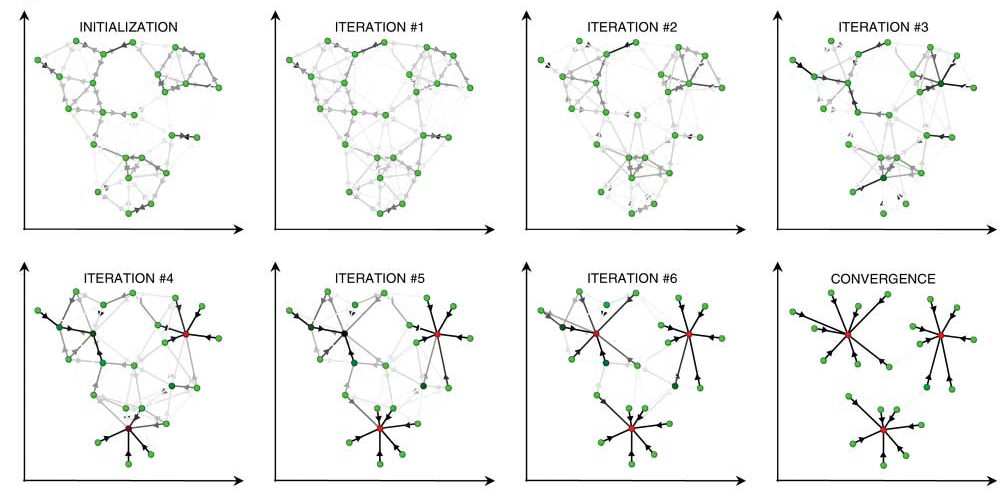
\includegraphics[width=500px]{./images/AP_frey.png}
\caption{Message passing between evolution over iteration.}
\end{figure}

\section{Hierarchical Affinity Propagation}

The affinity propagation algorithm can be generalized in a hierarchical
clustering algorithm. Let $L$ be the number of layers. All exemplars at layer
$l$ should also be exemplars at level $l -1$. Hence, number of exemplars
should decrease when going up the layers, and one exemplar at level $l$ can
either stay an exemplar at level $l + 1$ or chose another exemplar to be its
exemplar. Similarly, this can be expressed as the following ; if point $i$ isn't chosen as
exemplar at layer $l - 1$, ie, $e_{i}^{l - 1} = 0$, it then won't be clustered at
level $l$ ; if a point $i$ is an exemplar at level $l -1$ then it must choose
an exemplar at level $l$.\\

We can express the new constraints as follow:

\begin{itemize}
\item At level $1$, all points are clustered::
\begin{equation}
\sum_{j} h_{ij}^1 = 1
\end{equation}
\item At level $l$, only points that are exemplars at level $l - 1$ are
clustered.
\begin{equation}
\sum_{j} h_{ij}^l = e_i^{l-1}
\end{equation}

\item If a point is an exemplar at level $l$, then it is necessarily it's own
exemplar at this level.
\begin{equation}
e_j^l = h_{jj}^l = \max_i h_{ij}^l
\end{equation}
\end{itemize}

One could also imagine layer specific similarities $(s^l_{ij})$ and examplars
$(p^l_j)$. Therefore, the objective function to optimize is:

\begin{equation*}
\renewcommand{\arraystretch}{2}
\begin{array}{ccll}
\text{maximise} & & \sum_{i, j, l} s^l_{ij} h^l_{ij} + \sum_{j} p^l_j e^l_j \\
\text{subject to} &  & \sum_{j} h_{ij}^1 = 1 & j = 1, \dots, n\\
		  &  & e^l_{j} = h^l_{jj}, & j = 1, \dots, n\\
		  &  & \sum_{j} h_{ij}^l = e_i^{l-1}, & i = 1, \dots, n\\

\end{array}
\end{equation*}

To solve this optimization problem, two messages are passed up and down the
layers, in addition to the responsibilities and availabilities.

\begin{equation}
\tau_j^{l + 1} = p^l_j + r_{jj}^l + \sum_{k \neq j} \max (0, \rho^l_{jk})
\end{equation}

\begin{equation}
\phi_j^{l - 1} = \max_k (a_{jk}^l + s_{jk}^l)
\end{equation}

And the modified availabilities and responsabilities are:

\begin{equation}
a_{ij}^{l < L} = \begin{cases}
	    p_j + \phi_j^l + \sum_{k \neq j} \max(0, r_{kj}) &  i = j \\
	    \min ( 0, p_j + \phi_j^l + r_{jj} + \sum_{k \notin \{i, j\} } ) \max (0, r_{ij}) & i \neq j\\
	 \end{cases}
\end{equation}

\begin{equation*}
r_{ij}^{l > 1} = s_{ij}  + \min [ \tau_i^l, - \max_{k \neq j} (a_{ik} + s_{ik}) ]
\end{equation*}

The responsabilities for layer $l = 1$ and the availabilities for layer $l =
L$ are identical to the standard AP messages. \\

\cite{hap} shows that HAP outperforms both greedy message parsing algorithm,
and algorithm based on $k$-means with random restarts. Unfortunately, in a
small number of cases, HAP fails to converge. \cite{hap} suggests to run both
a greedy algorithm and the HAP, and to pick the results for which the
objective function is the lowest.

\begin{algorithm}[h]
  \SetLine
  initialization\;
  \For{iteration}{
    Compute $\tau_j^{l + 1} = p^l_j + r_{jj}^l + \sum_{k \neq j} \max (0, \rho^l_{jk}) $\;
    Compute $\phi_j^{l - 1} = \max_k (a_{jk}^l + s_{jk}^l)$\;
    \For{all layers}{
      Compute availabilities 
	$a_{ij}^{l < L} = \begin{cases}
	    p_j + \phi_j^l + \sum_{k \neq j} \max(0, r_{kj}) &  i = j \\
	    \min ( 0, p_j + \phi_j^l + r_{jj} + \sum_{k \notin \{i, j\} } \max
	    (0, r_{ij})) & i \neq j\\
	\end{cases}$  \;
       Compute responsibilities 
	$r_{ij}^{l > 1} = s_{ij}  + \min [ \tau_i^l, - \max_{k \neq j} (a_{ik} + s_{ik}) ]$\;

      }
  }
  Compute exemplars $e_i = \arg \max_{j} a_{ij} + s_{ij}$ \;
  \caption{Hierarchical Affinity Propagation}
\end{algorithm}

\section{Results}

\bibliography{ipol_hap}

\end{document}
%-------------------------------------------------------------------------------
